
%{{{ Preamble

\documentclass[journal,a4paper]{IEEEtran}
\hyphenation{op-tical net-works semi-conduc-tor}

%{{{ Packages

\usepackage[l2tabu,orthodox, abort]{nag}
\usepackage{fontspec}

\usepackage{microtype}
\frenchspacing

\usepackage{polyglossia}
\setdefaultlanguage{english}

\usepackage{graphicx}
\graphicspath{{../material/paper/}{../material/background/}}

\usepackage{minted}
\usepackage{lipsum}
\usepackage{url}
\usepackage{stfloats}
\fnbelowfloat




\makeatletter
\let\MYcaption\@makecaption
\makeatother
\usepackage[font=footnotesize]{subcaption}
\makeatletter
\let\@makecaption\MYcaption
\makeatother

%}}}


%{{{ New commands

%\newcommand{\source}[1]{{\caption{\tiny {\fontspec{ProFontWindows} {Source: #1} } } } }
\newcommand{\source}[1]{Source: #1}
%}}}


%{{{ Avebritations

\def\krste/{Krste Asanovi\'c}
\def\CC/{C\nolinebreak\hspace{-.05em}\raisebox{.4ex}{\tiny\textbf{+}}\nolinebreak\hspace{-.03em}\raisebox{.4ex}{\tiny\textbf{+}}}
%}}}



%}}}



\addto\captionsenglish{%
  \renewcommand\tablename{Listing}%
}











\begin{document}
%\setlength{\parindent}{0mm}

%{{{ Title, author, abstract and keywords

\title{RISC-V --- Architecture and Interfaces\\The RocketChip}


\author{Moritz~N\"oltner-Augustin\\%
University of Heidelberg, ZITI}
%	\IEEEcompsocitemizethanks{\IEEEcompsocthanksitem M. N\"oltner is enrolled at the University of Heidelberg and is currently pursuing a B.S. degree in applied informatics.\protect\\
%	E-mail: sh386@ix.urz.uni-heidelberg.de}%
%\thanks{Manuscript received January 6, 2015; revised January 12, 2015.}}%

% The paper headers
\markboth{Advanced Seminar ``Computer Engineering'', UNIVERSITY OF HEIDELBERG WT16/17}%
{Shell \MakeLowercase{\textit{et al.}}: RISC-V --- Architecture and Interfaces\\The RocketChip}

\maketitle

\begin{abstract}
	This paper gives a short overview of the RocketChip system-on-chip generator and how to use it.
\end{abstract}

% Note that keywords are not normally used for peerreview papers.
\begin{IEEEkeywords}
	RISC-V, RocketChip, Boom, SoC generator.
\end{IEEEkeywords}

%}}}

%{{{
\section{Introduction}
\IEEEPARstart{C}{omputer} technology has seen the rise and fall of many instruction set architectures (ISAs) over time.
Proprietary ISAs not only lead to fragmentation of the CPU market, but are also vulnerable to extinction when their proprietor companies run into financial troubles.
Along with design complexity and licensing issues, these considerations led \krste/ et al.\ to decide upon creating a new and free ISA for their next round of research projects at the University of California Berkeley (UCB).
This fifth reduced instruction set ISA developed at UCB, called RISC-V, is --unlike its predecessors-- not only meant for teaching but also actual implementation.
With three supported word-widths (32, 64 and 128 bits), RISC-V is aimed at all possible computational environments ranging from small embedded systems up to full scale supercomputers.
To facilitate widespread adoption, the ISA is licensed permissively, allowing use for academic and commercial use in open- and closed-source designs free of charge and now, roughly 4 years after its inception, RISC-V is used in a number of roles:

\begin{itemize}
	\item The LowRISC project aims to become the ``linux of the hardware word''
	\item SiFive and Open-V are creating custom silicon products
	\item ETH Zurich and Università di Bologna cooperate to create a state-of-the-art parallel microcontroller
	\item IIT Madras creates a processor
	\item NVIDIA will use the RISC-V ISA for the replacement of their Falcon processor
	\item UCB uses RISC-V processors for research purposes as well as for teaching
\end{itemize}
%}}}

%{{{
\section{RocketChip}
The UCB currently developes three lines of RISC-V processors, Sodor, Rocket and Boom.
Sodor is a collection of simple processors for use in lectures, Rocket is a scalar in-order processor for personal applications and Boom is a superscalar out-of-order processor for high performance applications.
All three are written in Chisel (Creating Hardware in a Scala Embedded Language), a hardware description language --as the name implies-- embedded in Scala.
Chisel allows compilation into three distinct target formats, the first of which is a cycle accurate \CC/ model for fast simulation and software development, the other targets are verilog code aimed at implementation in an FPGA or ASIC\@.
For Rocket and Boom there is a generator framework that can create a whole parametrised system around the processor cores, called RocketChip.
It will create one or more Rocket, Boom or custom cores, surround it with caches, optionally an FPU and accelerators to form one or more tiles. Then the tiles are connected to a TileLink network. The CPU is finished by adding TileLink to AXI4 converters to provide a well known bus interface to the outside world. Figure~\ref{rcov} shows a schematic of the generated system.

%{{{ RocketChip overview

\begin{figure}[!t]
	\centering
	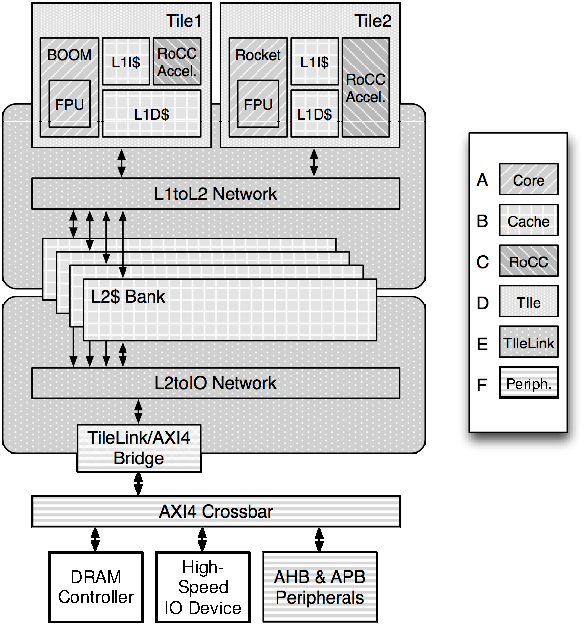
\includegraphics[width=3in]{rcov}
	\caption{Overview of the components of RocketChip.\newline\hspace{\linewidth}\source{Image taken from~\cite{rcgen}}.}
	\label{rcov}
\end{figure}
%}}}

\subsection{General Usage}
The RocketChip is maintained in a Git repository.
To build the default-configuration RocketChip, one only has to clone the repository, build the included GCC toolchain for RISC-V, and run ``\texttt{make}'' as shown in listing~\ref{rcclone}. For building a Boom-chip, the steps are identical except that one also has to checkout the ``\texttt{boom}'' branch of the same repository which then includes the Booms repo as a submodule.

%{{{ RocketChip Build Steps

\begin{table}
	\caption{Build steps for RocketChip.\newline\hspace{\linewidth}Source: Collected from~\cite{rc_github} and~\cite{boom_github}.}
	\begin{subtable}[b]{0.9\linewidth}
		\begin{minted}[fontsize=\small, gobble=3, tabsize=2]{bash}
			# $RC is some place in the file system
			cd $RC
			git clone \
			https://github.com/ucb-bar/rocket-chip.git
			cd rocket-chip
			git checkout boom # Only to build Boom
			git submodule update --init --recursive
		\end{minted}
		\caption{Downloading and initialising.}
		\label{rcclone}
	\end{subtable}
	\begin{subtable}[b]{0.9\linewidth}
		\begin{minted}[fontsize=\small, gobble=3, tabsize=2]{bash}
			cd $RC/riscv-tools
			export RISCV=/where/to/install/toolchain
			export PATH="${PATH}:$RISCV/bin"
			./build.sh # Takes about 45 min
		\end{minted}
		\caption{Building the RSCV-toolchain.}
		\label{rctoolchain}
	\end{subtable}
	\begin{subtable}[b]{0.8\linewidth}
		\begin{minted}[fontsize=\small, gobble=3, tabsize=2]{bash}
			cd $RC/emulator # Build the C++ simulator
			make run CONFIG=ExampleSmallConfig
			cd $RC/vsim     # Create the verilog code
			make -jN CONFIG=ExampleSmallConfig
		\end{minted}
		\caption{Building the SOC and a simulator. Substitute CONFIG=BOOMConfig when building a BOOM.}
		\label{rcmake}
	\end{subtable}
\end{table}
%}}}

If the environment variable RISCV is not set to point to a sane installation of the toolchain, the following build steps will fail, so the next part is building the RISCV-toolchain as shown in listing~\ref{rctoolchain}.


\subsection{Building a Configuration}
The makefile has a variable named ``\texttt{CONFIG}'' which is set to the name of a configuration.
A configuration is a set of configuration options that define the generated system.
Available configuration options can be found in \texttt{\$(RC)/src/main/scala/coreplex/Configs.scala}, and include for example:
%{{{ RocketChip config options

\begin{itemize}
	\item What core[s] (Rocket | BOOM | Custom)
	\item \#Tiles/Cores
	\item Cache configuration (Associativity, ECC, replacement policy)
	\item Debug hardware (\#Breakpoints, \#Performance Counters)
	\item What floating point unit
	\item What multiplication and division logic
	\item What atomic instructions
	\item Bootrom
	\item TileLink config
\end{itemize}
%}}}
These options are grouped into different build configurations which can be found in \texttt{\$RC/src/main/scala/rocketchip/Configs.scala}.
Building one of the pre-defined configurations is as simple as setting the \texttt{CONFIG} variable while \texttt{make}-ing the project. Listing~\ref{rcmake} shows the steps to build the emulator and the verilog source code for a certain RocketChip configuration.


\subsection{Creating a Configuration}
RocketChip configurations are written as scala code and inherit from the \texttt{Config} class defined in \texttt{\$RC/src/main/scala/config/Configs.scala}, which sets up some functionality including the '++' operator that is used to add the configuration options, or one of its child classes which already have some options set.
To evaluate the propagation of different configuration options into the generated verilog code, two new configurations differing in cache associativity and size were created as shown in listing~\ref{new-configs} using the configurations options listed in listing~\ref{config-options}.

%{{{ Config Options

\begin{table}
	\caption{Overview of the configuration system.}
	\begin{subtable}[b]{0.9\linewidth}
		\begin{minted}[fontsize=\small, gobble=3, tabsize=2]{scala}
			class BaseCoreplexConfig
							extends Config ((site, here, up) => {
				case CacheBlockBytes => 64
				case CacheName("L1D") => CacheConfig(
				nSets= 64,
				nWays= 4,
				rowBits= site(L1toL2Config).beatBytes*8,
				nTLBEntries= 8,
				cacheIdBits= 0,
				splitMetadata = false)
				...
			})
			...
			class WithL1ICacheSets(sets: Int)
					extends Config((site, here, up) => {
				case CacheName("L1I") =>
					up(CacheName("L1I"), site).copy(nSets = sets)
			})

			class WithCacheBlockBytes(linesize: Int)
					extends Config((site, here, up) => {
				case CacheBlockBytes => linesize
			})
		\end{minted}
		\caption{Extract of some of the configuration options found in \texttt{\$RC/src/main/scala/coreplex/Configs.scala}.}
		\label{config-options}
	\end{subtable}
	\begin{subtable}[b]{0.9\linewidth}
		\begin{minted}[fontsize=\small, gobble=3, tabsize=2]{scala}
			// Config with 2-way, 32 sets x 64 bytes/block cache
			// tag: 21 bits, index: 5 bits, WS: 4 bits, BS: 2 bits
			class DualCoreConfig2way extends Config(
				new WithNCores(2) ++ new WithL1ICacheWays(2)
				                  ++ new WithL1ICacheSets(32)
				                  ++ new WithCacheBlockBytes(64)
				                  ++ new WithL2Cache
				                  ++ new BaseConfig)

			// Config with 4-way, 64 sets x 32 byts/block cache
			// tag: 21 bits, index: 6 bits, WS: 3 bits, BS: 2 bits
			class DualCoreConfig4way extends Config(
				new WithNCores(2) ++ new WithL1ICacheWays(4)
				                  ++ new WithL1ICacheSets(64)
				                  ++ new WithCacheBlockBytes(32)
				                  ++ new WithL2Cache
				                  ++ new BaseConfig)
		\end{minted}
		\caption{Example of new RocketChip configurations defined in \texttt{\$RC/src/main/scala/rocketchip/Configs.scala}.}
		\label{new-configs}
	\end{subtable}
\end{table}
%}}}

\subsection{Analysis of configuration propagation}
The instruction cache parameters were chosen for their simple observability. Unlike for example the TileLink configuration options, the cache parameter only affect one verilog module, ICache\_icache, and are relatively simple to check by examining the SRAM memories that are instantiated.
For the 2-way configuration, the core of the cache can be expected to be two 32x21 bit tag SRAMs and two 32x512 bit (32x64 bytes) data SRAMs\footnote{\label{note-width}Or of course a configuration of smaller width but the same capacity}.
Likewise one would expect four 64x21 bit tag SRAMs and four 64*256 bit (64*32 bytes) data SRAMs\footnotemark[\ref{note-width}] for the 4-way configuration.

%{{{ Module ICache_icache

\begin{table}
	\caption{Extracts from the generated ICache\_icache Module.}
	\label{srams}
	\begin{subtable}[b]{0.9\linewidth}
		%2-way:
		%tag                   index WS   BS
		%XXXXXXXXXXXXXXXXXXXXX XXXXX XXXX XX
		\begin{minted}[fontsize=\small, gobble=3, tabsize=2]{verilog}
				// Instantiated once
				module tag_array(
					input  [4:0] RW0_addr,
					input   RW0_en,
					input   RW0_clk,
					input   RW0_wmode,
					input  [20:0] RW0_wdata_0,
					input  [20:0] RW0_wdata_1,
					output [20:0] RW0_rdata_0,
					output [20:0] RW0_rdata_1,
					input   RW0_wmask_0,
					input   RW0_wmask_1
				);
				reg [41:0] ram [31:0];
				...
				// Instantiated twice
				module _T_772(
					input  [7:0] RW0_addr,
					input   RW0_en,
					input   RW0_clk,
					input   RW0_wmode,
					input  [63:0] RW0_wdata,
					output [63:0] RW0_rdata
				);
				reg [63:0] ram [255:0];
		\end{minted}
		\caption{The instantiated SRAMs for the 2-way configuration.}
		\label{srams-2-way}
	\end{subtable}
	\begin{subtable}[b]{0.9\linewidth}
		%4-way:
		%tag                   index  WS  BS
		%XXXXXXXXXXXXXXXXXXXXX XXXXXX XXX XX
		\begin{minted}[fontsize=\small, gobble=3, tabsize=2]{verilog}
				// Instantiated once
				module tag_array(
					input  [5:0] RW0_addr,
					input   RW0_en,
					input   RW0_clk,
					input   RW0_wmode,
					input  [20:0] RW0_wdata_0,
					input  [20:0] RW0_wdata_1,
					input  [20:0] RW0_wdata_2,
					input  [20:0] RW0_wdata_3,
					output [20:0] RW0_rdata_0,
					output [20:0] RW0_rdata_1,
					output [20:0] RW0_rdata_2,
					output [20:0] RW0_rdata_3,
					input   RW0_wmask_0,
					input   RW0_wmask_1,
					input   RW0_wmask_2,
					input   RW0_wmask_3
				);
				reg [83:0] ram [63:0];
				...
				// Instantiated four times
				module _T_850(
					input  [7:0] RW0_addr,
					input   RW0_en,
					input   RW0_clk,
					input   RW0_wmode,
					input  [63:0] RW0_wdata,
					output [63:0] RW0_rdata
				);
				reg [63:0] ram [255:0];
		\end{minted}
		\caption{The instantiated SRAMs for the 4-way configuration.}
		\label{srams-4-way}
	\end{subtable}
\end{table}
%}}}

Looking at the generated code shown in listing~\ref{srams}, it can be verified, that indeed SRAMs of the expected capacities are created.
However the two and four tag SRAMs are merged into a big single two- and four-port SRAM respectively.
The data SRAMs use a narrower but deeper storage array, providing word-wise access but retaining the correct capacity. The required capacity per cache is the same for both configurations so the same SRAM gets instantiated.
The used SRAM verilog modules get created by the script \texttt{\$RC/vsim/vlsi\_mem\_gen} which per default generated behavioural descriptions of the requested SRAMs.
For an actual implementation, this script should be adapted to generate verilog wrappers for actually available SRAM blocks.
Since such an implementation will be forced to always use the next bigger (wider and/or deeper) available SRAM type, it might be interesting to dimension the cache organisation accordingly to maximise the cache parameters within the used SRAMs.






%}}}

%\lipsum

%{{{
\section{Conclusion}
%Both \twi\ and SPI are very mature, while still up-to-date bus systems for low-speed, low-complexity interconnection of integrated circuits.
%With their wide acceptance and when used as intended, both \twi\ and SPI are recommendable and reliable bus systems.

%}}}

\bigskip
%\vfill

%{{{
\begin{thebibliography}{1}
	\bibitem{rcgen}
	Asanovi\'c, Krste/Avizienis, Rimas/Bachrach, Jonathan et at. (2016)\\
	The Rocket Chip Generator.\\
	Technical Report No. UCB/EECS--2016--17, EECS Department, University of California, Berkeley.\\
	\url{http://www2.eecs.berkeley.edu/Pubs/TechRpts/2016/EECS--2016--17.html}\\

	\bibitem{rc_github}
	The RocketChip github pages\\
	\url{https://github.com/ucb-bar/rocket-chip}\\
	\url{https://github.com/ucb-bar/project-template}\\

	\bibitem{boom_github}
	The Berkeley Out Of Order Machine github page\\
	\url{https://github.com/ucb-bar/riscv-boom}\\


\end{thebibliography}
\enlargethispage{-5in}
%}}}


\end{document}
